\documentclass[border=6pt]{standalone}
\usepackage{tikz}
\usepackage{pgfplots}
\pgfplotsset{compat=1.18}
\usetikzlibrary{arrows.meta,positioning,shapes.geometric,fit,backgrounds,calc,decorations.pathreplacing,patterns,pgfplots.groupplots}
\tikzset{
  blk/.style={rectangle, rounded corners=2pt, draw=black!70, thick, fill=blue!6,
              minimum height=8mm, minimum width=20mm, align=center, font=\small},
  io/.style={rectangle, rounded corners=6pt, draw=black!70, thick, fill=green!8,
             minimum height=8mm, align=center, font=\small},
  proc/.style={rectangle, draw=black!70, thick, fill=orange!10, minimum height=8mm,
               align=center, font=\small},
  dec/.style={diamond, aspect=2, draw=black!70, thick, fill=yellow!15, align=center, font=\footnotesize},
  warnbox/.style={rectangle, rounded corners=2pt, draw=red!60!black, thick, fill=red!7,
                  minimum height=8mm, align=center, font=\small},
  oklbox/.style={rectangle, rounded corners=2pt, draw=green!45!black, thick, fill=green!8,
                 minimum height=8mm, align=center, font=\small},
  ar/.style={-{Latex[length=2mm]}, thick},
  arl/.style={-{Latex[length=2mm]}, thick, dashed, draw=black!55},
  lbl/.style={font=\footnotesize\itshape, text=black!60},
}
\definecolor{good}{RGB}{34,139,34}
\definecolor{bad}{RGB}{178,34,34}
\definecolor{warn}{RGB}{218,165,32}
\definecolor{pesblue}{RGB}{0,45,98}
\definecolor{complete}{RGB}{30,125,79}
\definecolor{partial}{RGB}{176,106,0}
\definecolor{blocked}{RGB}{166,43,43}
\begin{document}
% Canvas ~15.4 cm wide so it is included at ~0.89 scale; \scriptsize (7 pt)
% text prints at ~6.2 pt. Lane contents: outputs/E1_E14_FINAL_RESULTS_2026-09-19.md
% (sections 2-5, 9.1) and finish/Pending_Experiments.md terminal-state table;
% E1/E2/E5/E6/E9/E13 replacement cells: outputs/finish_pending_2026-09-27/<lane>/result.json.
% E14: 2271/4428 = 0.51287 (campaign rule: 2 unjudged rows count as failures);
% the official scorer's 0.51310 = 2271/4426 drops the 2 unjudged rows.
% E10: 88/97 = 0.90722 (public_portfolio_2026-09-05/results.json score).
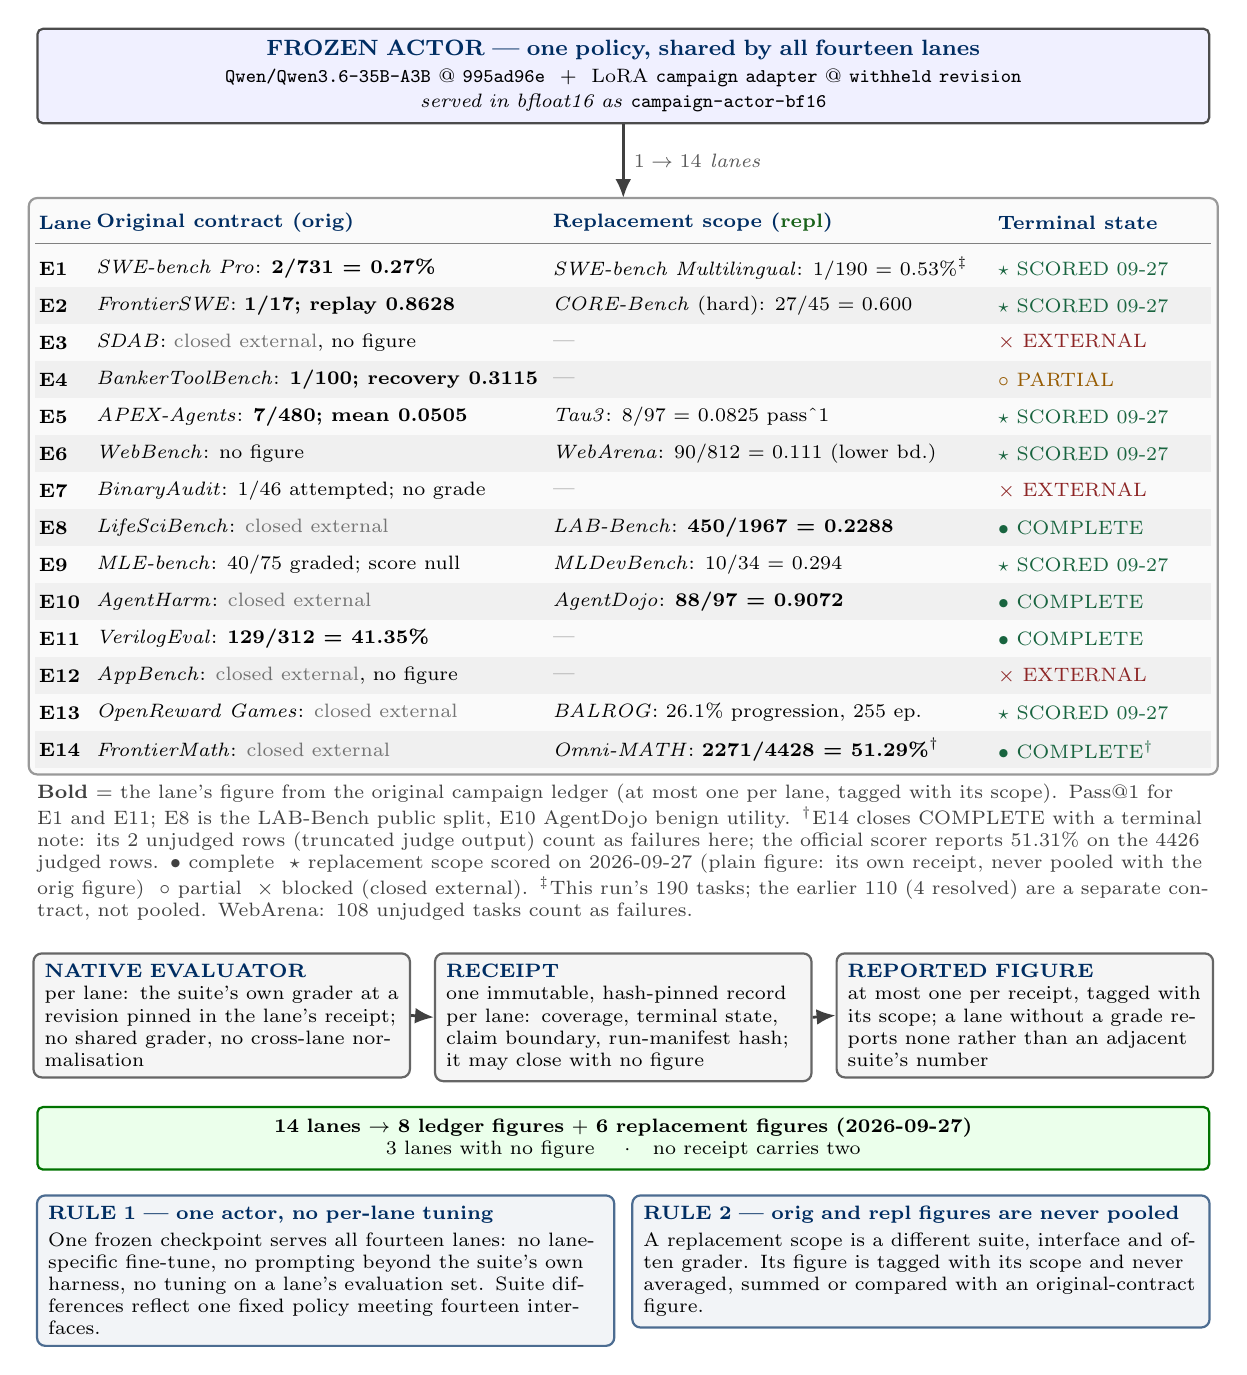
\begin{tikzpicture}[x=1cm,y=1cm,
  cell/.style={anchor=west, font=\scriptsize, inner sep=0pt, align=left},
  hdr/.style={anchor=west, font=\scriptsize\bfseries, text=pesblue, inner sep=0pt},
  rail/.style={rectangle, rounded corners=3pt, draw=black!60, thick, fill=black!4,
               align=left, inner sep=4pt, text width=4.5cm, minimum height=1.55cm,
               font=\scriptsize, anchor=north},
  rulebox/.style={rectangle, rounded corners=3pt, draw=pesblue!70, thick, fill=pesblue!5,
                  align=left, inner sep=4pt, font=\scriptsize, anchor=north},
  sar/.style={-{Latex[length=2.4mm,width=2.0mm]}, line width=1.0pt, draw=black!75},
]

% 1. FROZEN ACTOR --------------------------------------------------------
\node[rectangle, rounded corners=2pt, draw=black!70, thick, fill=blue!6,
      text width=14.6cm, inner sep=4pt, font=\scriptsize, align=center] (actor) at (7.55,0)
  {{\footnotesize\bfseries\color{pesblue}FROZEN ACTOR --- one policy, shared by all fourteen lanes}\\[2pt]
   \texttt{Qwen/Qwen3.6-35B-A3B} @ \texttt{995ad96e} \ $+$ \ LoRA
   \texttt{campaign adapter} @ \texttt{withheld revision}\\[1pt]
   \textit{served in bfloat16 as} \texttt{campaign-actor-bf16}};
\draw[sar] (actor.south) -- (7.55,-1.55)
  node[midway, right, font=\scriptsize\itshape, text=black!65] {$1 \rightarrow 14$ lanes};

% 2. LANE TABLE: original contract vs replacement scope --------------------

\fill[black!2, rounded corners=3pt] (0.0,-1.55) rectangle (15.1,-8.87);
\draw[black!40, thick, rounded corners=3pt] (0.0,-1.55) rectangle (15.1,-8.87);
\node[hdr] at (0.12,-1.86) {Lane};
\node[hdr] at (0.85,-1.86) {Original contract ({\color{pesblue}orig})};
\node[hdr] at (6.65,-1.86) {Replacement scope ({\color{good!70!black}repl})};
\node[hdr] at (12.3,-1.86) {Terminal state};
\draw[black!50] (0.08,-2.13) -- (15.02,-2.13);
\node[cell, font=\scriptsize\bfseries] at (0.12,-2.445) {E1};
\node[cell] at (0.85,-2.445) {\emph{SWE-bench Pro}: \textbf{2/731 = 0.27\%}};
\node[cell] at (6.65,-2.445) {\emph{SWE-bench Multilingual}: 1/190 = 0.53\%$^{\ddagger}$};
\node[cell] at (12.3,-2.445) {\textcolor{complete!80!black}{$\star$\ SCORED 09-27}};
\fill[black!6] (0.08,-2.680) rectangle (15.02,-3.150);
\node[cell, font=\scriptsize\bfseries] at (0.12,-2.915) {E2};
\node[cell] at (0.85,-2.915) {\emph{FrontierSWE}: \textbf{1/17; replay 0.8628}};
\node[cell] at (6.65,-2.915) {\emph{CORE-Bench} (hard): 27/45 = 0.600};
\node[cell] at (12.3,-2.915) {\textcolor{complete!80!black}{$\star$\ SCORED 09-27}};
\node[cell, font=\scriptsize\bfseries] at (0.12,-3.385) {E3};
\node[cell] at (0.85,-3.385) {\emph{SDAB}: {\color{black!55}closed external}, no figure};
\node[cell] at (6.65,-3.385) {{\color{black!45}---}};
\node[cell] at (12.3,-3.385) {\textcolor{blocked!85!black}{$\times$\ EXTERNAL}};
\fill[black!6] (0.08,-3.620) rectangle (15.02,-4.090);
\node[cell, font=\scriptsize\bfseries] at (0.12,-3.855) {E4};
\node[cell] at (0.85,-3.855) {\emph{BankerToolBench}: \textbf{1/100; recovery 0.3115}};
\node[cell] at (6.65,-3.855) {{\color{black!45}---}};
\node[cell] at (12.3,-3.855) {\textcolor{partial!85!black}{$\circ$\ PARTIAL}};
\node[cell, font=\scriptsize\bfseries] at (0.12,-4.325) {E5};
\node[cell] at (0.85,-4.325) {\emph{APEX-Agents}: \textbf{7/480; mean 0.0505}};
\node[cell] at (6.65,-4.325) {\emph{Tau3}: 8/97 = 0.0825 pass\^{}1};
\node[cell] at (12.3,-4.325) {\textcolor{complete!80!black}{$\star$\ SCORED 09-27}};
\fill[black!6] (0.08,-4.560) rectangle (15.02,-5.030);
\node[cell, font=\scriptsize\bfseries] at (0.12,-4.795) {E6};
\node[cell] at (0.85,-4.795) {\emph{WebBench}: no figure};
\node[cell] at (6.65,-4.795) {\emph{WebArena}: 90/812 = 0.111 (lower bd.)};
\node[cell] at (12.3,-4.795) {\textcolor{complete!80!black}{$\star$\ SCORED 09-27}};
\node[cell, font=\scriptsize\bfseries] at (0.12,-5.265) {E7};
\node[cell] at (0.85,-5.265) {\emph{BinaryAudit}: 1/46 attempted; no grade};
\node[cell] at (6.65,-5.265) {{\color{black!45}---}};
\node[cell] at (12.3,-5.265) {\textcolor{blocked!85!black}{$\times$\ EXTERNAL}};
\fill[black!6] (0.08,-5.500) rectangle (15.02,-5.970);
\node[cell, font=\scriptsize\bfseries] at (0.12,-5.735) {E8};
\node[cell] at (0.85,-5.735) {\emph{LifeSciBench}: {\color{black!55}closed external}};
\node[cell] at (6.65,-5.735) {\emph{LAB-Bench}: \textbf{450/1967 = 0.2288}};
\node[cell] at (12.3,-5.735) {\textcolor{complete!80!black}{$\bullet$\ COMPLETE}};
\node[cell, font=\scriptsize\bfseries] at (0.12,-6.205) {E9};
\node[cell] at (0.85,-6.205) {\emph{MLE-bench}: 40/75 graded; score null};
\node[cell] at (6.65,-6.205) {\emph{MLDevBench}: 10/34 = 0.294};
\node[cell] at (12.3,-6.205) {\textcolor{complete!80!black}{$\star$\ SCORED 09-27}};
\fill[black!6] (0.08,-6.440) rectangle (15.02,-6.910);
\node[cell, font=\scriptsize\bfseries] at (0.12,-6.675) {E10};
\node[cell] at (0.85,-6.675) {\emph{AgentHarm}: {\color{black!55}closed external}};
\node[cell] at (6.65,-6.675) {\emph{AgentDojo}: \textbf{88/97 = 0.9072}};
\node[cell] at (12.3,-6.675) {\textcolor{complete!80!black}{$\bullet$\ COMPLETE}};
\node[cell, font=\scriptsize\bfseries] at (0.12,-7.145) {E11};
\node[cell] at (0.85,-7.145) {\emph{VerilogEval}: \textbf{129/312 = 41.35\%}};
\node[cell] at (6.65,-7.145) {{\color{black!45}---}};
\node[cell] at (12.3,-7.145) {\textcolor{complete!80!black}{$\bullet$\ COMPLETE}};
\fill[black!6] (0.08,-7.380) rectangle (15.02,-7.850);
\node[cell, font=\scriptsize\bfseries] at (0.12,-7.615) {E12};
\node[cell] at (0.85,-7.615) {\emph{AppBench}: {\color{black!55}closed external}, no figure};
\node[cell] at (6.65,-7.615) {{\color{black!45}---}};
\node[cell] at (12.3,-7.615) {\textcolor{blocked!85!black}{$\times$\ EXTERNAL}};
\node[cell, font=\scriptsize\bfseries] at (0.12,-8.085) {E13};
\node[cell] at (0.85,-8.085) {\emph{OpenReward Games}: {\color{black!55}closed external}};
\node[cell] at (6.65,-8.085) {\emph{BALROG}: 26.1\% progression, 255 ep.};
\node[cell] at (12.3,-8.085) {\textcolor{complete!80!black}{$\star$\ SCORED 09-27}};
\fill[black!6] (0.08,-8.320) rectangle (15.02,-8.790);
\node[cell, font=\scriptsize\bfseries] at (0.12,-8.555) {E14};
\node[cell] at (0.85,-8.555) {\emph{FrontierMath}: {\color{black!55}closed external}};
\node[cell] at (6.65,-8.555) {\emph{Omni-MATH}: \textbf{2271/4428 = 51.29\%}$^{\dagger}$};
\node[cell] at (12.3,-8.555) {\textcolor{complete!80!black}{$\bullet$\ COMPLETE$^{\dagger}$}};
\node[cell, anchor=north west, text width=14.9cm, text=black!75] (note) at (0.1,-8.990)
  {\textbf{Bold} $=$ the lane's figure from the original campaign ledger (at most one per lane, tagged with its scope).
   Pass@1 for E1 and E11; E8 is the LAB-Bench public split, E10 AgentDojo benign utility.
   $^{\dagger}$E14 closes COMPLETE with a terminal note: its 2 unjudged rows (truncated judge output)
   count as failures here; the official scorer reports $51.31\%$ on the 4426 judged rows.
   $\bullet$~complete \ $\star$~replacement scope scored on 2026-09-27 (plain figure: its own receipt, never pooled with the orig figure)
   \ $\circ$~partial \ $\times$~blocked (closed external).
   $^{\ddagger}$This run's 190 tasks; the earlier 110 (4 resolved) are a separate contract, not pooled. WebArena: 108 unjudged tasks count as failures.};

% 3. GOVERNANCE RAILS ------------------------------------------------------
\node[rail] (R1) at ([yshift=-4mm]note.south -| 2.45,0)
  {{\bfseries\color{pesblue}NATIVE EVALUATOR}\\ per lane: the suite's own grader at a
   revision pinned in the lane's receipt; no shared grader, no cross-lane normalisation};
\node[rail] (R2) at ([yshift=-4mm]note.south -| 7.55,0)
  {{\bfseries\color{pesblue}RECEIPT}\\ one immutable, hash-pinned record per lane:
   coverage, terminal state, claim boundary, run-manifest hash; it may close with no figure};
\node[rail] (R3) at ([yshift=-4mm]note.south -| 12.65,0)
  {{\bfseries\color{pesblue}REPORTED FIGURE}\\ at most one per receipt, tagged with its
   scope; a lane without a grade reports none rather than an adjacent suite's number};
\draw[sar] (R1.east) -- (R2.west);
\draw[sar] (R2.east) -- (R3.west);

\node[rectangle, rounded corners=2pt, draw=green!45!black, thick, fill=green!8,
      text width=14.6cm, inner sep=4pt, font=\scriptsize, align=center, anchor=north]
  (tally) at ([yshift=-3mm]R2.south)
  {{\bfseries 14 lanes $\rightarrow$ 8 ledger figures $+$ 6 replacement figures (2026-09-27)}\\
   3 lanes with no figure \quad$\cdot$\quad no receipt carries two};

% 4. THE TWO GOVERNING RULES ----------------------------------------------
\node[rulebox, text width=7.05cm] (rule1) at ([yshift=-3mm,xshift=-3.78cm]tally.south)
  {{\bfseries\color{pesblue}RULE 1 --- one actor, no per-lane tuning}\\[1.5pt]
   One frozen checkpoint serves all fourteen lanes: no lane-specific fine-tune, no
   prompting beyond the suite's own harness, no tuning on a lane's evaluation set.
   Suite differences reflect one fixed policy meeting fourteen interfaces.};
\node[rulebox, text width=7.05cm] (rule2) at ([yshift=-3mm,xshift=3.78cm]tally.south)
  {{\bfseries\color{pesblue}RULE 2 --- orig and repl figures are never pooled}\\[1.5pt]
   A replacement scope is a different suite, interface and often grader. Its figure
   is tagged with its scope and never averaged, summed or compared with an
   original-contract figure.};

\end{tikzpicture}
\end{document}
